

\section{Existing Protocols for Local DP}

Apart from R.R., several L.D.P. protocols have been implemented during the years, with many of them being widely used by companies in order to protect users' data. One of the most famous protocols is \emph{RAPPOR}([15]), created by Google, and being currently used in the Chrome browser for the company to provide useful info to its users without compromising their privacy. Also, Apple has created ts own protocol of L.D.P., and utilize it in their products. 

However, we are not going to focus on those protocols moving forward, than the ones presented in [10], a paper which introduces many algorithms for L.D.P., each one with different perturbation techniques and suitable for different circumstances.

During this chapter we are going to give a definition of each algorithm, implement it using Python, and compare the accuracy results produced by those protocols, just like during our testings of the G.D.P. models. Each protocol has two parts: the \emph{users} and the \emph{aggregator}. For the users we must each time define the following functions:

\begin{itemize}
    \item $Encode()$: Encodes the true value that the user wants to report
    \item $Perturb()$: Perturbs the encoded value, in order to produce the random value that will be reported
\end{itemize}

For the aggregator we must each time define the  $Aggregate()$ function, that collects the reported random values of the users, and produces the results according to the model.

\subsection{Basic RAPPOR}
As mentioned earlier, RAPPOR is a protocol created by Google. Its simpler form, Basic RAPPOR is used in Chrome, where it collects answers to questions such as the user's home page. The protocol's functions are the following:

\textbf{Encoding:} $Encode(v) = A_0$, where $A_0$ is a d-bit vector, such that: $A_0[v] = 1$ and $A_0[i] = 0$ for every $i \neq v$. 

\textbf{Perturbation:} The perturbation consists of 2 steps: the permanent and the instantaneous. The permanent one is carried out only one time, and is the following: 

\begin{equation*}
    Pr[A_1[i] = 1] =
	\begin{cases}
		1 - \frac{1}{2}f & \mbox{if } A_0[i]=1 \\
		\frac{1}{2}f & \mbox{ otherwise}
			\end{cases}
\end{equation*}

The instantaneous step is carried out every time a user reports a value, and is defined as:

\begin{equation*}
    Pr[A_2[i] = 1] =
	\begin{cases}
		p & \mbox{if } A_1[i]=1 \\
		q & \mbox{ otherwise}
			\end{cases}
\end{equation*}

We observe from the above functions, that the user must define the $f, p $ and $q$ parameters. Google suggests that we set $f = \frac{1}{2}$ or $\frac{1}{4}$, and $p = 0.75$, thus $q = 0.25$. During our testings, those exact parameters were used. 


\subsection{Random Matrix Projection}
In [14], a protocol with a random matrix projection is proposed, introducing an additional setup step.

\textbf{Setup:} A random and uniform matrix is generated before any encoding, with it being public and drawn as: $\Phi \in \{-\frac{1}{m}, \frac{1}{m}\}^{m \times d}$, where $m$ and $d$ are user defined. In our testings, we opt to set $m = 5$ and $d = 10$.

\textbf{Encoding:} When it comes down to encoding, the function used is the following: $Encoding = (r,x)$, where $r$ is uniformly randomly selected from the range of m, and $x$ is the v-th element of the r-row of the random matrix.

\textbf{Perturbation}: The perturbation function is defined as following: 
\begin{align*}
 Perturb(r,x) = (r, b\cdot c \cdot m \cdot x) 
\end{align*}
 where
\begin{equation*}
    b =
	\begin{cases}
		1 & \mbox{with } p = \frac{e^\epsilon}{e^\epsilon + 1} \\
		-1 & \mbox{with } q = \frac{1}{e^\epsilon + 1}			
	\end{cases}
\end{equation*}
and $c = \frac{e^\epsilon +1}{e^\epsilon -1}$

\textbf{Aggregation:} Given all the tuples reported by $j$ users in the form $(r, y)$, the estimation for the i-th value of the dataset, is produced by 
\begin{align*}
\sum_{j} y^j \cdot \Phi[r^j,i]
\end{align*}

\subsection{Pure Protocols}

The following protocols are presented in [10], and are called "pure" protocols, because of the way they aggregate the data produced by the user. For each one of them, we should define a $Support()$ function, that indicates for each value of the possible outcomes, the reported values that are supported. Thus, with the notation $\sum_{j} Support(y^j)$, we mean the sum of all the supported values of the y-th element of the dataset.

Also, for a protocol to be pure, two probabilities must be defined, $p^*$ and $q^*$, where the first notes the probability that the true value is supported by an element $y$, and the second one the probability of another value is supported by the element $y$. The protocol is pure if and only if $p^* > q^*$.

If a protocol is pure, the estimation of the total reported values for an element of the dataset $i$, is the following:

\begin{align}
    \text{Estimation} = \frac{\sum_{j} 1_{support(y^j)}(i) - nq*}{p^* - q^*}
\end{align}
where $j$ denotes the j-th user reporting their value, and $n$ the total size of the vector of the reported values.


\subsubsection{Direct Encoding}

This protocol is the natural method of extending the Randomized Response, without the limitation of 2 possible answers. 

\textbf{Encoding:} The protocol does not feature an encoding procedure, thus 

\begin{align*}
    Encode(v) = v
\end{align*}

\textbf{Perturbation:} The perturbation is based on the epsilon setting given by the user, and its function is defined as following:

\begin{equation*}
    Pr[Perturb(x) = i] =
	\begin{cases}
    	p = \frac{e^\epsilon}{e^\epsilon + d - 1} & \mbox{if } i = x \\
    	q = \frac{1}{e^\epsilon + d - 1} & \mbox{if } i \neq x 
	\end{cases}
\end{equation*}

where $d$ the size of the dataset of the possible answers, $x$ the true value and $i$ the value selected.

\textbf{Aggregation:} The protocol is pure with $p^* = p$, $q^* = q$ and $Support(i) = i$, thus the predicted results for each of the dataset's values can be calculated from the Equation 4.1.

We observe that this protocol strongly depends on the size of the dataset of the possible answers, thus when the dataset size increases, the protocol becomes less accurate, due to the decreased probability of selecting the truth. Moreover, for the D.E. protocol, all the false values have the same probability to get chosen, a rather disturbing detail for a query such as a person's age. We will return to these thoughts on later sections.

\subsubsection{Histogram Encoding}

An other protocol presented is Histogram Encoding, where an input when having $d$ options is encoded as a $d$-length vector.

\textbf{Encoding:} The encoding function is for the protocol is

\begin{align*}
    Encoding(v) = [0, 0, \dots, 1, \dots, 0]
\end{align*}

where only the v-th element of the vector is equal to 1.

\textbf{Perturbation:} The result of perturbing the encoded vector, is a new vector $B'$, s.t.: 

\begin{align*}
    B'[i] = B[i] + Lap(\frac{2}{\epsilon})
\end{align*}
where $Lap()$ denotes the noise drawn from the Laplace distribution, where


\begin{align*}
    Pr[Lap(\beta) = x] = \frac{1}{2\beta}e^{\frac{-|x|}{\beta}}
\end{align*}

\textbf{Aggregation:} Several methods are proposed for aggregating the results created by the H.E. protocol, but as mentioned by the authors, the best one is called \emph{Thresholding with H.E.}, where a threshold value is introduced in order to decide what to keep from the reported values. The support function is altered as following:

\begin{align*}
    Support(B) = \{v | B[v] > \theta\}
\end{align*}
thus, if a noisy output is grater than theta, is set to support the corresponding value. According to the authors, the optimal value for θ is in the range of $(\frac{1}{2}, 1)$. During the testings that are going to be conducted, we are going to use a threshold of $\frac{2}{3}$.


Comparing this protocol to D.E., we observe that is solves the problem of the dependence of the noise drawn by the number of options to choose from. In H.E., no matter how large the domain size is, the noise solely depends on the epsilon value chosen by the user. Thus, when having a large domain size, it is clear that we should prefer the H.E. protocol over D.E.

\subsection{Unary Encoding}

The last protocol that is going to take part in the accuracy testings, is the Unary Encoding method, a further exploration of the Basic RAPPOR. It is a unique protocol, as the user does not set the level of privacy using epsilon, but by giving two probabilities, $p$ and $q$ and the epsilon value is computed using those two parameters.

\textbf{Encoding:} Exactly like in the H.E. method:
\begin{align*}
Encoding(v) = [0, 0, \dots, 1, \dots, 0] 
\end{align*}
where only the v-th element of the vector is equal to 1.

\textbf{Perturbation:} This step is different than those that we already saw, and is carried out using the following function:


\begin{equation*}
    Pr[B'[i] = i] =
	\begin{cases}
    	p  & \mbox{if } B[i] = 1 \\
    	q & \mbox{if } B[i] = 0 
	\end{cases}
\end{equation*}

The epsilon value is decided given $p$ and $q$, and is defined as following:

\begin{align*}
    \epsilon = ln(\frac{p\cdot(1-q)}{(1-p)\cdot q})
\end{align*}

\textbf{Aggregation:} The Support function is once again altered, as in the U.E. protocol is defined as following:

\begin{align*}
    Support(B) = \{i | B[i] = 1\}
\end{align*}

and of course, $p^* = p$ and $q^* = q$, in order to make the protocol pure. As for the choice of $p$ and $q$, we opt to choose $p = \frac{1}{2}$, and $q = \frac{1}{e^\epsilon + 1}$.

\section{Testings}

\subsection{Setup}

Now that all those protocols where introduced, we are going to compare them in order to decide which is better to use when wanting to apply L.D.P. in a dataset. We are going to use a dataset that was created using random values, but corresponds to the age of a group of people. The distribution of the values of the dataset is shown in the histogram in \textbf{Figure 4.2. }

\begin{figure}[!htb]\centering
    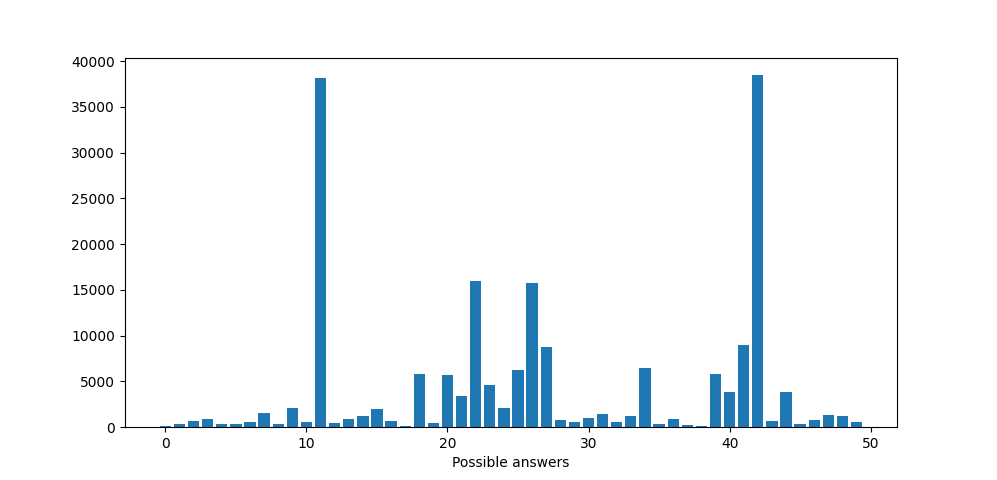
\includegraphics[width=1\textwidth]{images/true_answers_ldp.png}
    \caption{True Answers for the Dataset of LDP}
\end{figure}

Each user will report one of these 50 values, and the aggregator of each protocol will gather the data given, and try to re-create this histogram in the best manner possible.

\subsection{Goal}

We want to decide which protocols behaves better, thus a number of different metrics will be used. The main focus of our testings will be the vectors that the aggregators provide, which we will compare with each other, as well as with the vector containing the true answers. In a similar way as our G.D.P. testings, we are going to run the protocols for different values of epsilon, and different number of users used. The second one is extremely important in L.D.P., as we mentioned earlier that many protocols struggle with a small number of input, as the noise drawn is significant. 

With respect to the choice of metrics, we are going to use the \emph{Manhattan Distance}, known as the $l1$-norm, as well as the \emph{Kantorovic Distance}, explained in 3.2.5.1.

\subsection{Epsilon Measurements}

The first comparison between the protocols will be with a changing epsilon value, in order to observe how they behave for lower and higher values of the privacy setting. During these testings, all of the users of the dataset were used (approximately 20 thousand), and each run of each protocol was carried out 10 times, just like in other testings, in order to eliminate the danger of drawing extreme values of noise.

First, we are going to run all the protocols and compare them using the Manhattan Distance. The results are shown in \textbf{Figure 4.3.}


\begin{figure}[!htb]\centering
    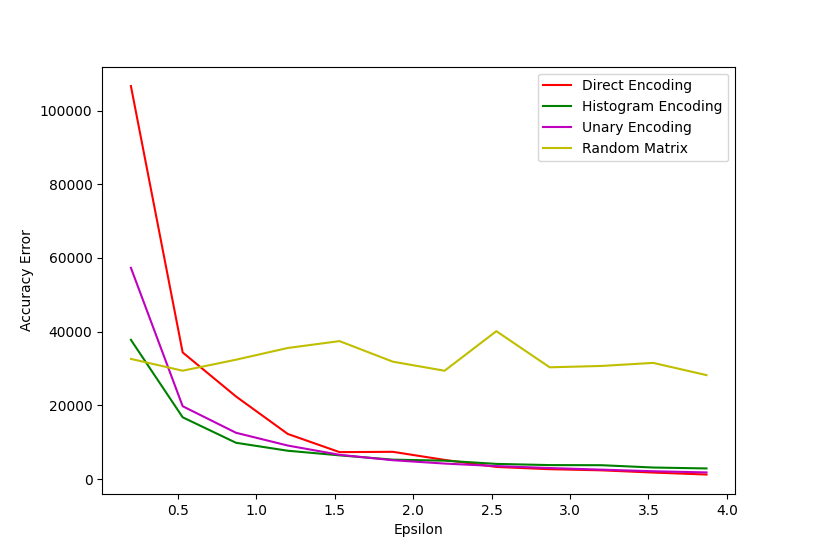
\includegraphics[width=1\textwidth]{images/epsilon_others_l1.png}
    \caption{Epsilon Measurements compared by Manhattan Distance}
\end{figure}


We gather many useful observations from the graph:

\begin{itemize}
    \item The Random Matrix protocol does not function as expected, as \emph{its accuracy does not follow the logarithmic curve we are used to when epsilon increases.} However, for small values of ε, its results are acceptable, and some times even better than the pure protocols.
    \item \emph{The pure protocols behave in a similar way}, with the error stabilizing when epsilon gets higher than 2.5. 
    \item \emph{The Direct Encoding protocol was the worst behaviour among the pure ones}, with its error being extremely high for epsilon values lower than 1.  This is mainly due to the fact that when ε gets too small, the probability of telling the truth gets significantly low, thus creating a big error in accuracy.
    \item \emph{The optimized U.E. protocol has the best behaviour} in comparison to the other protocols tested.
\end{itemize}

Next up, we are going to run the same testings, but this time using the Kantorovich metric. We expect the protocols to behave even worse, because of the identity of the metric: the Kant. metric pays attention to the distance of the reported answer from the true one. The current protocols do not take into account the distance of the two answers, thus the metric will probably report a higher error. The results of the runs are shown in \textbf{Figure 4.4.}

\begin{figure}[!htb]\centering
    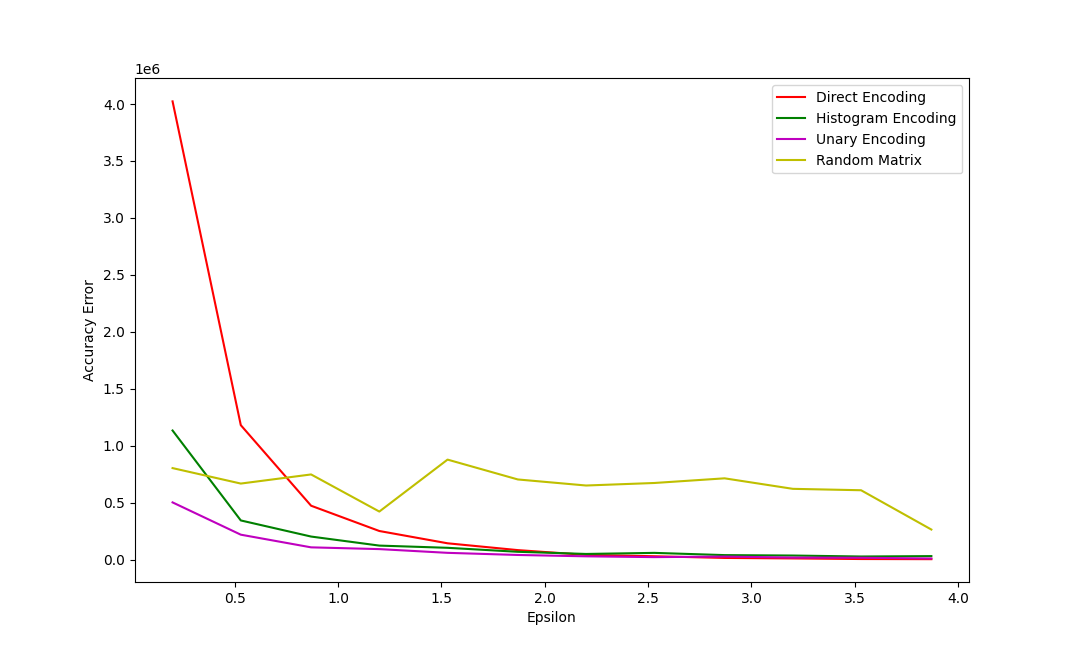
\includegraphics[width=1\textwidth]{images/epsilon_others_kant.png}
    \caption{Epsilon Measurements compared by Kantorovic Distance}
\end{figure}


As we expected, the protocols produce a higher error, with the D.E. being the worst among them, especially for lower values of epsilon. This is a rather alarming notice, in which we will come back in Section 4.6.


\subsection{Increasing number of users}


The second experiment that we will conduct is the accuracy error depending on the number of users used during the survey covered by the protocol. In the definition of L.D.P. the observation of the need of lots of users was made, and it is now time that we examine it. We are going to use a \emph{fixed epsilon value}, one that our protocols behave similarly for (at least the pure ones, in which we will focus our research moving forward). Our epsilon value that we are going ot used will be fixed and equal to 1.5.

We are going to run the protocols and compare them using the Manhattan Distance. Additionally, we are each time going to divide the result of the metric with the number of users participated, as the simple error is going to increase when the users increase. Hence, this division is going to give us the error depending on the size of our domain. The results are shown in \textbf{Figure 4.5.}

\begin{figure}[!htb]\centering
    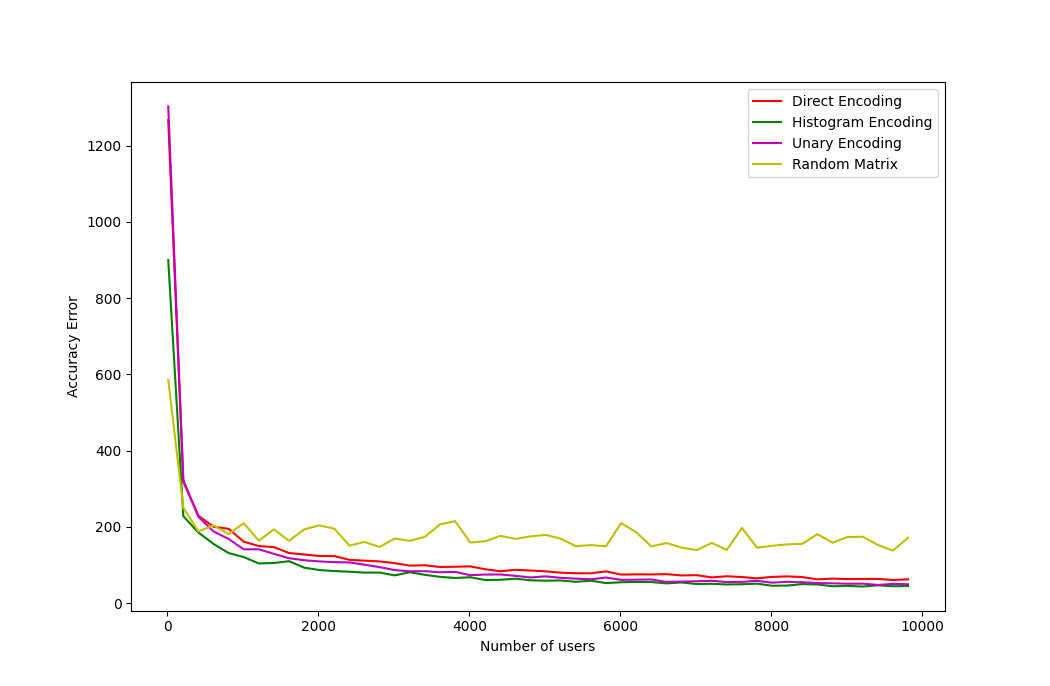
\includegraphics[width=1\textwidth]{images/nusers_others_l1.png}
    \caption{Increasing n. of users compared by Manhattan Distance}
\end{figure}

The results confirm the allegations made after explaining the definition of L.D.P.: When the number of participants in a survey is low, the error produced is very high. Every protocol has similar behaviour, as we can see that for fewer than 1000 users the relative error is even 6 times larger than for more than 1000 users. Actually, as we can see from the graph, the turning point is around 2000 users: the relative error drops and stabilizes after this number of participants. 

An other observation made, is that the protocol with the best behaviour during our epsilon measurements (Unary Encoding), is the worst one in the low users testings. This of course gets better as the number of participants rises, and eventually beats the other protocols when it comes down to relative accuracy error. 

Next up, we are going to perform the same testings while comparing the protocols with the Kantorovich metric. The results are shown in \textbf{Figure 4.6}.

\begin{figure}[!htb]\centering
    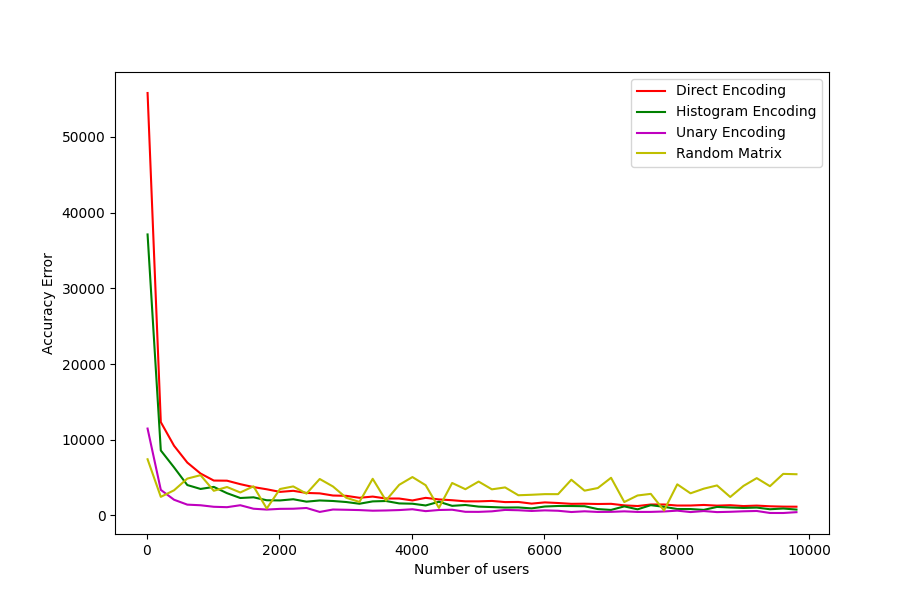
\includegraphics[width=1\textwidth]{images/nusers_others_kant.png}
    \caption{Increasing n. of users compared by Kantorovich Distance}
\end{figure}

The results for a low number of users differ a lot from the runs with the $l1$ distance as a metric. Here, the D.E. method has obviously the worst behaviour, and the U.E. method the best. We can even claim that U.E. seems to solve our problem of high accuracy error. However, no one of those protocols takes into account the distance of the reported answer from the true one, thus it makes sense that the Kantorovich metric produces a huge amount of accuracy error.

That fact, triggered our thoughts, on what could possibly be done in order to reduce that problem. The thoughts made on this subject are analyzed in the next chapter, by creating a new L.D.P. protocol, sensitive to the distance between the true and the reported values.